\documentclass[a4paper, 11pt]{article}
\usepackage[left=2.5cm,right=2.5cm,top=3cm,bottom=3cm,a4paper]{geometry}
\usepackage{kotex}
\usepackage{color}
\usepackage{enumitem}
\usepackage[cmyk, dvipsnames, svgnames]{xcolor}
\usepackage{graphicx}
\DeclareGraphicsExtensions{.pdf,.png,.jpg}
\usepackage[onehalfspacing]{setspace}
\setstretch{2.0}
\usepackage[colorlinks,urlcolor=blue,filecolor=magenta]{hyperref}
\usepackage{url}
\usepackage{graphicx,subfigure}






\title{\textbf{\Huge오목 한글 설명서}}
\author{\textbf{\LARGE5조}}
\begin{document}
	
	\maketitle
	
	\vspace{6cm}
	\begin{center}
		\textbf{\large20134824 김민석    (gominvkd94@hanmail.net)}\\
		\textbf{\large20134852 허정건    (ini080@naver.com)}\\
		\textbf{\large20134867 이현문    (lhm3561@naver.com)}\\
	\end{center}
	
	
	
	
	\maketitle
	\newpage
	\thispagestyle{empty}        
	\mbox{}
		
	\begin{center} 
		\textbf{\Huge목차}\\
	\end{center}
	\vspace{0.5cm}
\section{프로그램 선택 이유 .................................................................. 3}
	\vspace{0.5cm}
	\section{프로그램 설명 ........................................................................ 4}
	\begin{itemize}
		\item 소개 및 목표
	\end{itemize}
	
	\section{게임 소개 ............................................................................... 5}
		\begin{itemize}
		\item 각 실행 화면
	\end{itemize}

	
	\section{게임 설명 ............................................................................... 7}
	\begin{itemize}
		\item 게임 룰
		\item 게임 조작법
	\end{itemize}
	
	
	
	
	\section{버그 ...................................................................................... 10}
	
	\vspace{0.5cm}
	\section{개선할 점 ............................................................................... 11}

	
	\vspace{0.5cm}
	\section{GitHub 협력자료 ................................................................... 12}
	
   \newpage
	\title{\textbf{\Huge1. 프로그램 선택 이유}}\\
	
\textbf{	{\Large
		\begin{itemize}
			\item 현재 수 많은 오픈소스중에 설명서를 만듦에 있어 평소 우리가 자주 사용하지 않는 프로그램 보다 더 익숙하고 쉽게 접근할 수 있는 프로그램을 찾아 설명서를 만들어 보자는 생각에서 부터 오픈소스를 찾게되었다.\vspace{2cm}
			\item 평소 게임을 좋아하는 우리 팀은 자연스럽게 게임에 대한 오픈소스를 찾게되었고 그로부터 우리나라의 전통놀이인 오목게임의 오픈소스를 찾게되었다. 누구나 쉽고 익숙하게 즐길 수 있는 전통놀이 오목의 설명서를 만들면서 오목게임도 할 수 있고,설명서를 만들어 다른 사람에게 도움도 줄 수 있어 일석이조라고 생각하여  이 프로그램을 선택하게 되었다.
		\end{itemize}
	}
	}


	\newpage
	\title{\textbf{\Huge2. 프로그램 설명}}\\
	\textbf{
	\begin{itemize}
		\item \LARGE소개 
	\end{itemize}
	{\Large
	본 프로그램은 네이버 블로거 dnpc7848 에 의해 개발 되었으며, 현재 모든 소스를 오픈하고 수정과 배포에 제한을 두지 않고 있다.\\
	현재 다음 링크에서 쉽게 다운로드 받아 사용, 수정이 가능하다\\
	\url{http://blog.naver.com/dnpc7848/220895826336} 
	\vspace{3cm}
	}
	\begin{itemize}
		\item \LARGE목표
	\end{itemize}
	{\Large
		본 프로그램에서 일반 룰, 고모쿠 룰, 렌주 룰  이 세 가지 룰에 대해 각 룰을 선택하여 실행하고, AI 모드를 통해 인공지능 상대와 게임을 즐기며 또한 남녀노소 가리지 않고 누구나 쉽게 오목을 접하여 배우기 위함에 목표를 둔다
	}}
	\newpage
	\title{\textbf{\Huge3. 게임 소개}}\\
\begin{figure}[h] %%% t: top, b: bottom, h: here
	\begin{center}
		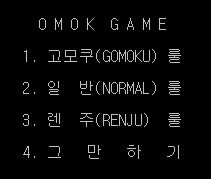
\includegraphics[width=0.5\linewidth]{first.png}
	\end{center}
	\label{fig:long}
	\label{fig:onecol}
\end{figure}
\begin{center}
	\textbf{{\Large 1. 룰 선택 화면\\}}
	\textbf{{\normalsize 원하는 룰 선택 \\}}
	\vspace{1.5cm}
\end{center}

\begin{figure}[h] %%% t: top, b: bottom, h: here
	\begin{center}
		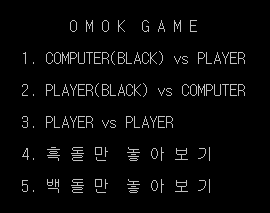
\includegraphics[width=0.5\linewidth]{second.png}
	\end{center}
	\label{fig:long}
	\label{fig:onecol}
\end{figure}
\begin{center}
	\textbf{{\Large 2. 플레이어 선택 화면\\}}
	\textbf{{\normalsize 원하는 상대 선택 \\}}
\end{center}

	\newpage
\begin{figure}[h] %%% t: top, b: bottom, h: here
	\begin{center}
		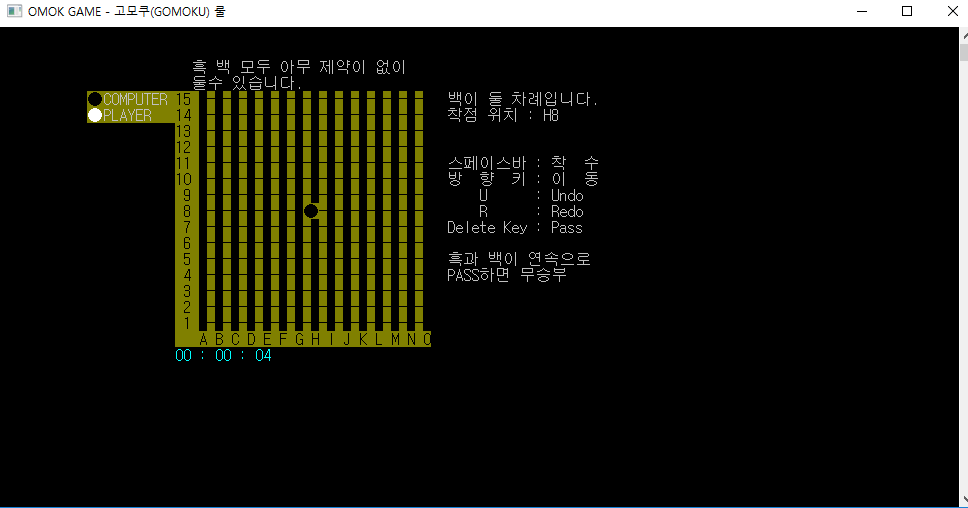
\includegraphics[width=0.8\linewidth]{third.png}
	\end{center}
	\label{fig:long}
	\label{fig:onecol}
\end{figure}
\begin{center}
	\textbf{{\Large 3. 게임 실행 화면\\}}
	\textbf{{\normalsize 게임 시작! \\}}
	\vspace{0.5cm}
\end{center}

\begin{figure}[h] %%% t: top, b: bottom, h: here
	\begin{center}
		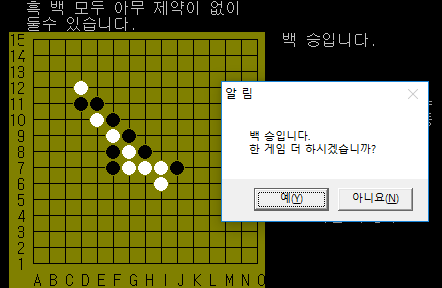
\includegraphics[width=0.8\linewidth]{4th.png}
	\end{center}
	\label{fig:long}
	\label{fig:onecol}
	
\end{figure}

\begin{center}
	\textbf{{\Large 4. 게임 결과\\}}
	\vspace{0.3cm}
	\textbf{{\normalsize 이겼닭! \tiny 오늘 저녁은 치킨이닭!  \\}}
\end{center}

 \newpage
\title{\textbf{\Huge4. 게임 설명 }
	\vspace{0.5cm}
	
	\textbf{\quad\Large1)게임룰}
	\begin{figure}[h]
		\begin{center}
			\subfigure{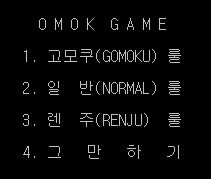
\includegraphics[width=0.35\linewidth]{OM_RuleSELECT.png}}
			\vspace{0.3cm}
			\textbf{\\\large고모쿠룰 일반룰 렌주룰 중 하나를 선택하여 플레이}
			\vspace{3.2cm}  	
			\begin{flushleft}
			\textbf{\qquad\large1.1)고모쿠 룰}	
			\end{flushleft}
			
			
			\subfigure{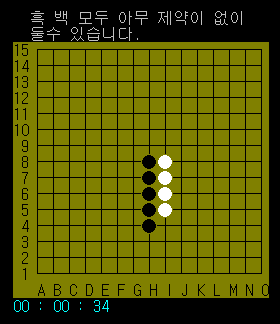
\includegraphics[width=0.35\linewidth]{komoku.png}}
			\vspace{0.5cm}
			\textbf{\large\\아무런 제약이 없는 오목으로 공식에서는 잘 사용하지 않음}
		
		\end{center}
	\end{figure}
	
	
	
	
	\newpage
	\textbf{\quad\large1.2)일반 룰}
	\begin{figure}[h]
		\begin{center}
			\subfigure{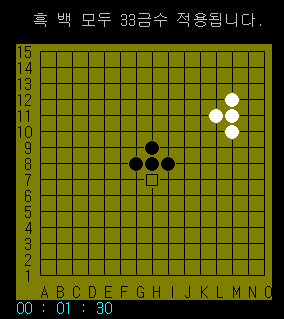
\includegraphics[width=0.30\linewidth]{normal.png}}
			
			\vspace{0.3cm}
		\textbf{\large\\일상적으로 가볍게 대전할 때 가장 많이 사용되는 룰. 일단 3-3은 흑, 백 모두 금지되나 여기서 2개의 라인의 양 끝, 즉 4개의 끝 중 하나라도 막혀있으면 금지수가 아니다. \qquad 4-4에서 4가 하나 띄워져 있더라도 금지이다.}
			\end{center}
	\end{figure}
\vspace{2cm} 	


		
		\textbf{\quad\large1.3)렌주 룰}
		\begin{figure}[h]
			\begin{center}
			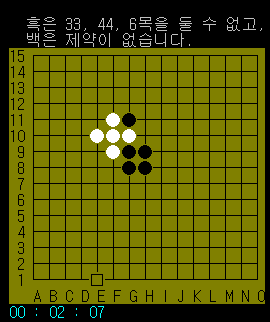
\includegraphics[width=0.35\linewidth]{renju.png}
				\vspace{0.3cm}
		\textbf{\large\\흑만 3-3, 4-4가 금지된다. \\(단, 4 또는 3과 동시에 5도 만들 수 있는 상황이라면 가능하다)}
		\end{center}
	\end{figure}
	
	
	
	
	\newpage
	\textbf{\title{\Large4.2 게임조작법} }\\
	
	
	\begin{figure}[h] %%% t: top, b: bottom, h: here
		\begin{center}
			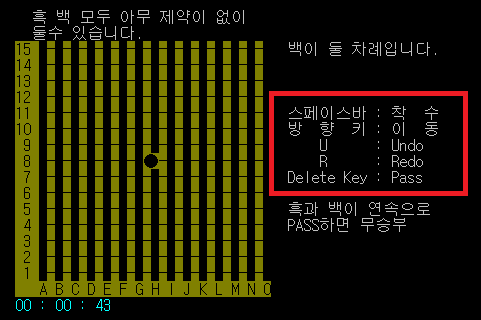
\includegraphics[width=0.7\linewidth]{OM_5.png}
		\end{center}
		\vspace{1.0cm}
		
		
	\begin{center}
		
	
		\textbf{\large4.2.1 스페이스바 \\}
		내 차례일 경우, 원하는 위치에 스페이스바를 눌러 착수\\
		\vspace{0.5cm}
		
		\textbf{\large4.2.2 방향키 \\}
		\qquad↑ : 위쪽으로 한칸 이동 \\
		\qquad↓ : 아래쪽으로 한칸 이동 \\
		\qquad← : 왼쪽으로 한칸 이동 \\
		\qquad→ : 오른쪽으로 한칸 이동 \\
		\vspace{0.5cm}
		
		\textbf{\large4.2.3 U \\}
		\qquad이미 착수된 돌을 다시 되돌리는 기능\\
		\vspace{0.5cm}
		
		\textbf{\large4.2.4 R \\}
		\qquad다시 두고 싶을 때 이미 착수된 돌을 되돌리는 기능\\ 
		\vspace{0.5cm}
		
		\textbf{\large4.2.5 Delete Key \\}
		\qquad 내 턴을 무시하고 다음 턴으로 넘기는 기능 \\
	\end{center}
	\end{figure}

 \newpage
\title{\textbf{\Huge5. 버그 }
	
		\vspace{1cm}
	{\large
\textbf{1. 구현된 3가지 룰을 선택해도 모두 '일반 룰'로 진행되는 버그.}
	
\textbf{2. 게임 결과 창  표시 후 첫 화면으로 돌아가는 것이 아닌 프로그램 종료 현상.}
	
\textbf{3. 육(6)목 이상을 나열 한 경우, 룰을 무시하고 승리로 간주되는 현상. }
\vspace{0.4cm}

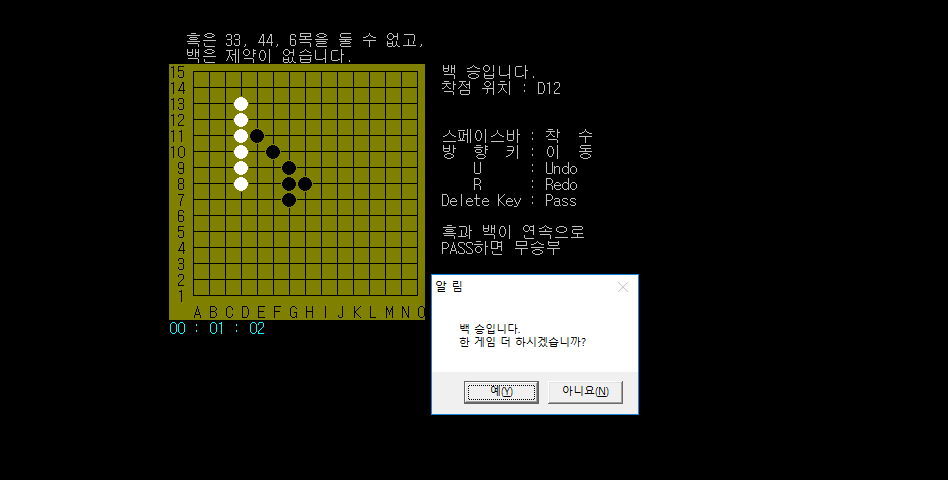
\includegraphics[width=1.0\linewidth]{5th.png}
	
\textbf{4. 조작키 설명 중 U(Undo)와 R(Redo) 둘다 같은 '되돌리기' 기능을 수행하면서}
  \textbf{\quad 각각 다른 키로 구현.}
 	
\textbf{5. 첫 화면으로 되돌아가는 'ESC' 기능이 룰 선택 화면에서는 적용이 되지않음.}
}
	\vspace{3cm}
\newpage
	\title{\textbf{\Huge6. 개선할 점 }
		
	\vspace{1cm}
		
	{\large		
		
\textbf{ 1. 게임 시작 시 항상 시작 돌이 H8 위치가 아닌 랜덤위치에서 시작 될 수 있게 수정\\}

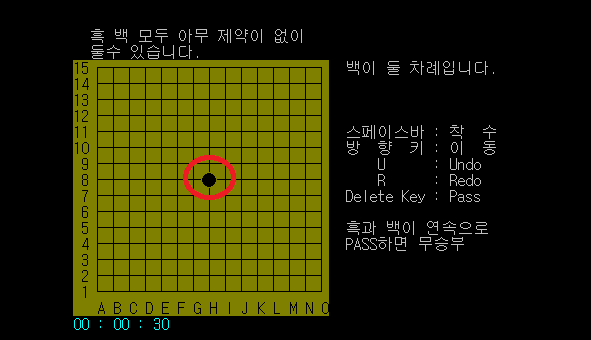
\includegraphics[width=1.0\linewidth]{6th.png}
		
\textbf{2. 결과 화면 승리자  '흑돌 승' 대신, 사용자 승리 로 표시}
		
\textbf{3. 조작키 설명 중 Delete Key 기능인 PASS를 더 쉽게 이해하기 위해 DRAW로 수정 }
		
\textbf{4. 제한시간을 두어 게임에 긴장감 조성이 필요}
		
\textbf{5. 마지막으로 둔 돌 위치를 강조하여 헷갈리지 않게 할 필요}
}

\newpage

	\title{\textbf{\Huge7. GitHub 협력자료 }
		
	\vspace{2cm}
		\includegraphics[width=1.0\linewidth]{network.png}
	\begin{center}
		\textbf{\Large Network Graph} 
	\end{center}

\vspace{3.5cm}
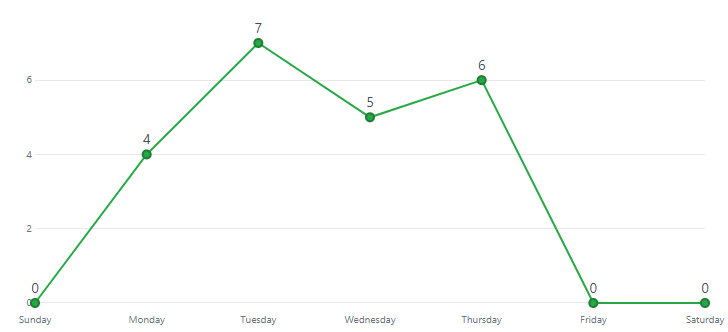
\includegraphics[width=0.9\linewidth]{commit.png}
\begin{center}
	\textbf{\Large Commit Graph} 
\end{center}

\vspace{0.5cm}
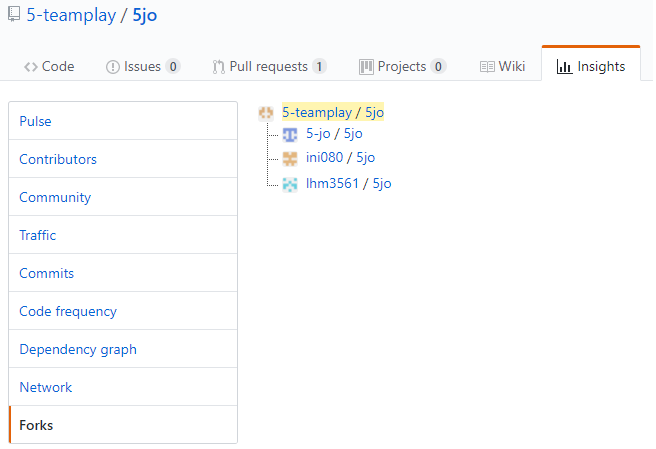
\includegraphics[width=1.0\linewidth]{fork.png}
\begin{center}
	\textbf{\Large Fork State} 
\end{center}
		
\end{document} 